
\begin{table*}[t]
\small
\centering
    \begin{tabular}{|c|c|c|c||c||c|c|c|c||c|c|c|c|}
 
        \hline
          Method & Anon. & Resour. &  Aug. & OntoNotes & T1-p &  T1-a & Avg & $\mid$ Diff $\mid$ & T2-p & T2-a & Avg & $\mid$ Diff $\mid$  \\
          \hline
           \UW &&&&{\bf 67.7}&{\bf 76.0}&49.4& 62.7&26.6* 
           &{\bf 88.7}&75.2 & 82.0 &13.5*\\
           \UW & \checkmark &&&66.4&73.5 & 51.2 &62.6&21.3*
           & 86.3 & 70.3&78.3&16.1* \\
           \UW & \checkmark & \checkmark &&66.5 &67.2&59.3&{63.2}&7.9*
           &81.4&82.3&81.9&0.9 \\
           \UW &\checkmark  & & \checkmark &66.2&65.1&59.2&62.2&5.9*
           &86.5&{\bf 83.7}&{\bf 85.1}& 2.8* \\
           \UW & \checkmark & \checkmark & \checkmark &66.3 &63.9&{\bf 62.8}&{\bf 63.4}&{\bf 1.1}
           &81.3&{ 83.4}&82.4&{\bf 2.1} \\
          \hline
          \hline
           \Berkeley &&&&{\bf 61.7}& {\bf 66.7} &56.0&{61.4}&10.6*&{\bf 73.0}&57.4&65.2&15.7* \\
           \Berkeley & \checkmark &&&61.3 &65.9&56.8&61.3&9.1*&72.0&58.5&65.3&13.5* \\
           \Berkeley & \checkmark & \checkmark &&61.2 &61.8&{\bf 62.0}&{\bf 61.9}&{\bf 0.2}&67.1&63.5&65.3&3.6 \\
           \Berkeley & \checkmark &  &\checkmark& 61.0&65.0&{57.3}&61.2&{7.7*}&{ 72.8}&{ 63.2}&{68.0}&{9.6*} \\
              \Berkeley & \checkmark & \checkmark &\checkmark& 61.0 &62.3&{60.4}&61.4&{1.9*}&{71.1}&{\bf 68.6}&{\bf 69.9}&{\bf 2.5} \\
          \hline
          \hline
           \Stanford &&&&57.0&76.7&37.5&57.1 & 39.2* &50.5 & 29.2& 39.9 & 21.3*\\
           
         % 10 & Stanford & \checkmark &&&&& \\
         
        \hline
    \end{tabular}
    \vspace{-10pt}

    \caption{\small F1 on OntoNotes and WinoBias development set. WinoBias results are split between Type-1 and Type-2 and in pro/anti-stereotypical conditions. * indicates the difference between pro/anti stereotypical conditions is significant ($p < .05$) under an approximate randomized test~\cite{graham2014randomized}. Our methods eliminate the difference between pro-stereotypical and anti-stereotypical conditions (Diff), with little loss in performance (OntoNotes and Avg). }
    \label{tab:results}
   % \vspace{-10pt}

\end{table*}



\begin{table*}[t]
\small
\centering
    \begin{tabular}{|c|c|c|c||c||c|c|c|c||c|c|c|c|}
 
        \hline
          Method & Anon. & Resour. &  Aug. & OntoNotes & T1-p &  T1-a & Avg & $\mid$ Diff $\mid$ & T2-p & T2-a & Avg & $\mid$ Diff $\mid$  \\
          \hline
           \UW &&&&{\bf 67.2}&{\bf 74.9}&47.7&61.3&27.2* 
           &{\bf 88.6}&77.3 & {\bf 82.9} &11.3*\\
           \UW & \checkmark & \checkmark & \checkmark &66.5 &62.4&{\bf 60.3}&{\bf 61.3}&{\bf 2.1}
           &78.4&{\bf 78.0}& 78.2 &{\bf 0.4} \\
          \hline
          \hline
           \Berkeley &&&&{\bf 64.0}& {\bf 62.9} &58.3&{60.6}&4.6*&{\bf 68.5}&57.8& 63.1 & 10.7* \\
           \Berkeley & \checkmark & \checkmark &\checkmark& 63.6 &62.2&{\bf 60.6}& {\bf 61.4}& {\bf 1.7} &{\bf 70.0}&{\bf 69.5}&{\bf 69.7}&{\bf 0.6} \\
          \hline
          \hline
           \Stanford &&&&58.7&72.0&37.5& 54.8 & 34.5* & 47.8 & 26.6 & 37.2 & 21.2*\\
           
         % 10 & Stanford & \checkmark &&&&& \\
         
        \hline
    \end{tabular}
    \vspace{-10pt}

    \caption{\small F1 on OntoNotes and Winobias test sets. Methods were run once, supporting development set conclusions.}
    \label{tab:test_results}
\vspace{-10pt}
\end{table*}

%%KW: Talk about the new dataset we collect and provide data statistics

In this section, we highlight two sources of gender bias in co-reference systems that can cause them to fail \dataset: training data and auxiliary resources and propose strategies to mitigate them.
%We first, look at bias coming directly from training data.
%Then we consider bias from auxiliary resources.

%analyze the coreference resolution corpus and existing systems and show that both the corpus and the models are biased. 
%To simplify the analysis, we consider only the binary gender in this work.
%However, the proposed approach can be applied to other types of biases. 
%Besides this, we propose a new winograd dataset which can be used as a benchmark to analyze the gender bias issue in the coreference systems.

\subsection{Training Data Bias}
\label{sub:ccb}

% We conduct several analyses on the training corpus to estimate how bias the data is. 
% We first demonstrate the common words that co-refer with male and female pronouns reveal bias.
% We then show that data set is imbalanced. 
% There are more male entities than female entities across the whole corpus.
% Finally, we show that there are several job titles that mostly corefer with male pronouns. 

% Table~\ref{tab:words} lists the most frequent 15 words co-refering with gender pronouns (e.g., ``he'',``his'', ``she'', ``her'').
% We use the following procedure to detect the words that have a strong co-relation with either male or female: we first obtain the coreference clusters in each document and extract the heads of all the mentions in the cluster.  Table~\ref{tab:words} shows the number of co-occurrence of male/female words~\footnote{male-words: [``he'', ``his'']; female-words: [``she'', ``her'']} with those heads.
%  Most of the words in this table are intrinsically gender-related. However, phrases such as ``lord'' and ``president'' occur in the top-15 male-related words while in female part, there is no such gender neutral word. These results show that some gender neural words corefer with male pronouns frequently, risking being bias. 

% \begin{table}[thbp]
% \centering
%     \begin{tabular}{|l|c|}
%         \hline
%          \bf Gender & \bf  Top-15 related words  \\
%           \hline
%          \multirow{3}{*}{Male}  &  he, his, him, i, jesus,  \\
%          & god, you, me, my, man, \\
%           & christ, \textbf{lord}, \textbf{president}, son, himself     \\
%          \hline
%         \multirow{3}{*}{Female} &   she, her, i, you, woman, \\
%          & my, me, wife, your, daughter, \\
%         & mother, herself, girl, clinton, mary \\
%         \hline
%     \end{tabular}
%     \caption{ Top-15 co-occurred words for different genders in training dataset. Most of the words are gender inherent. However in male part, titles such as ``lord'' and ``president'' appear but in female part, there are no such words. }
%     \label{tab:words}
% \end{table}
%\vspace{-5pt}
\paragraph{Bias in OntoNotes 5.0}
Resources supporting the training of co-reference systems have severe gender imbalance. 
In general, entities that have a mention headed by gendered pronouns (e.g.``he'', ``she'') are over 80\% male.\footnote{To exclude mentions such as ``his mother'', we use Collins head finder~\cite{collins2003head} to identify the head word of each mention, and only consider the mentions whose head word is gender pronoun.}
Furthermore, the way in which such entities are referred to, varies significantly. 
Male gendered mentions are more than twice as likely to contain a job title as female mentions.\footnote{We pick more than  900 job titles from a gazetteer. %\url{https://sourceforge.net/p/gate/code/HEAD/tree/gate/trunk/plugins/ANNIE/resources/gazetteer/jobtitles.lst}
}
Moreover, these trends hold across genres.

\vspace{-5pt}
\paragraph{Gender Swapping}
To remove such bias, we construct an additional training corpus where all male entities are swapped for female entities and vice-versa.
Methods can then be trained on both original and swapped corpora.
%in the OntoNotes corpus.
This approach maintains non-gender-revealing correlations while eliminating correlations between gender and co-reference cues.

We adopt a simple rule based approach for gender swapping. 
First, we anonymize named entities using an automatic named entity finder~\cite{lample2016neural}. Named entities are replaced consistently within document (i.e. ``Barak Obama ... Obama was re-elected.'' would be annoymized to ``E1 E2 ... E2 was re-elected.'' ).
Then we build a dictionary of gendered terms and their realization as the opposite gender by asking workers on Amazon Mechnical Turk to annotate all unique spans in the OntoNotes development set.\footnote{Five turkers were presented with anonymized spans and asked to mark if it indicated male, female, or neither, and if male or female, rewrite it so it refers to the other gender.}
Rules were then mined by computing the word difference between initial and edited spans.
Common rules included ``she $\rightarrow$ he'', ``Mr.'' $\rightarrow$ ``Mrs.'', ``mother'' $\rightarrow$ ``father.''
Sometimes the same initial word was edited to multiple different phrases: these were resolved by taking the most frequent phrase, with the exception of ``her $\rightarrow$ him'' and ``her $\rightarrow$ his'' which were resolved using part-of-speech.
Rules were applied to all matching tokens in the OntoNotes. We maintain anonymization so that cases like ``John went to his house'' can be accurately swapped to ``E1 went to her house.''
%To build the gender-reversed datasets, we asked Amazon Mechanical Turk to identify if a span in the coreference chain is related to male or female. 
%If it is , we then ask them to exchange it to the corresponding span with the other gender. For example, ``a waiter'' in the original corpus will be changed to ``a waitress'' in the new dataset. To get rid of the influence of names, we first anonymize the whole dataset.




% As the current  model is built on a male-biased dataset, it is difficult to for the model to get much information about female instances, for example, the model now learns ``leader'' only relates to male but has nothing to do with female. 
% %If we can  make the model learn the relation between ``leader'' and female, we can somehow reduce the bias. 
% %To calibrate the gender bias in coreference systems, we propose a data Aggregate  Re-Train (ART) algorithm  based on gender-reversed datasets. 
% %This approach aims at neutralizing the ability of a model to tell the difference between genders. 
% The ART approach is described as follows: First, we generate a gender-reversed training dataset using the same procedure as we did for the deployment set described in the previous section. 
% Then, we use the union set of the original corpus and the gender-reversed corpus as the new training set.
% Because the new training corpus is gender neutral, the models retrained on this corpus tend to be less affected by gender bias.
% For example, in the original corpus, the noun phrase ``the leader'' is exclusively referred using a male pronoun. Therefore, the model learns that female pronouns can not be used to refer to ``the leader''. However, in the new training data, both male and female pronouns refer to ``the leader''. Therefore, the model trained on the new corpus can identify female leaders. 
\subsection{Resource Bias}
%\vspace{-5pt}
\paragraph{Word Embeddings}
Word embeddings are widely used in NLP applications however recent work has shown that they are severely biased: ``man'' tends to be closer to ``programmer'' than ``woman''~\cite{BCWS16,CBN17}.
Current state-of-art co-reference systems build on word embeddings and risk inheriting their bias. %some co-ref systems that also use word embeddings.
To reduce bias from this resource, we replace GloVe embeddings with debiased vectors~\cite{BCWS16}.
%When the coreference resolution system is built on such word embeddings, it will  also be influenced by such stereotype.
\vspace{-5pt}
\paragraph{Gender Lists}
While current neural approaches rely heavily on pre-trained word embeddings, previous feature rich and rule-based approaches rely on corpus based gender statistics mined from external resources~\cite{Bergsma:06}.
Such lists were generated from large unlabeled corpora using heuristic data mining methods. %. and have been provided with co-reference training data since \my{XXX}. 
 These resources provide counts for how often a noun phrase is observed in a male, female, neutral, and plural context.
To reduce this bias, we balance male and female counts for all noun phrases.




%Besides the above data augmentation method, we also propose another Debiased Re-Train (DRT) approach to help mitigate the gender bias in the coreference resolution systems. With this method, we just need to replace the previous word embeddings in the coreference model to a debiased version without changing other parts of the model. 

%We also combine the above two methods together to calibrate the systems, which will be called the DART method. 



%We first show that the corpus is gender imbalanced and contains more male entities than female entities.
%We define the male and female entities to be the cluster of mentions containing at least one male pronoun (e.g., ``he'', ``his'', or ``him'') and female pronoun, respectively.
%We then count the total numbers of male and female entities in the entire corpus. %For simplicity, we convert 
%all words in the documents to lowercase. 
%In the following, we use ``\#male entities : \#female entities'' to represent the number of male and female entities in the corpus. 
%In the training and development corpus, male clusters occur four times more often than female cluster.
% Furthermore, female co-reference chains contain 3 times fewer mentions than male chains.
%$3393:787$. 
%There are about four times more male entities than female entities.
%The gender ratio in development corpus is $441:111$.
%Similar to the training corpus, approximately $80\%$ of entities with gender are male.
%As we can see the corpus is gender imbalanced and there are many more male entities than female.

%We are also interested in analyzing how many male and female entities in each document. 
%Figure~\ref{fig:his_cluster} shows a histogram of numbers of male and female entities. Fig.~\ref{fig:his_cluster} shows that most documents in both training and development corpus contain male entities, while a majority of documents do not contain any female entities (> 1,600).
%There are 45 documents having more than 10 male entities while only 7 documents contain more than 10 female entities in the training dataset.
%Also more than 1600 files having no female clusters while only about 780 files without male clusters.
%Both Fig.~\ref{fig:his_clu_train} and \ref{fig:his_clu_dev} show that most documents will have more male entities than female ones.

%We can see in both datasets, most documents have  less than 5 gender-related clusters.  For example, in Fig.~\ref{fig:his_clu_train}, almost all the documents have less than 10 clusters related to female, but one document can have as most as 34 male clusters. 

% \begin{figure*}[thbp]
%     \centering
%     \begin{subfigure}[b]{0.45\textwidth}
%         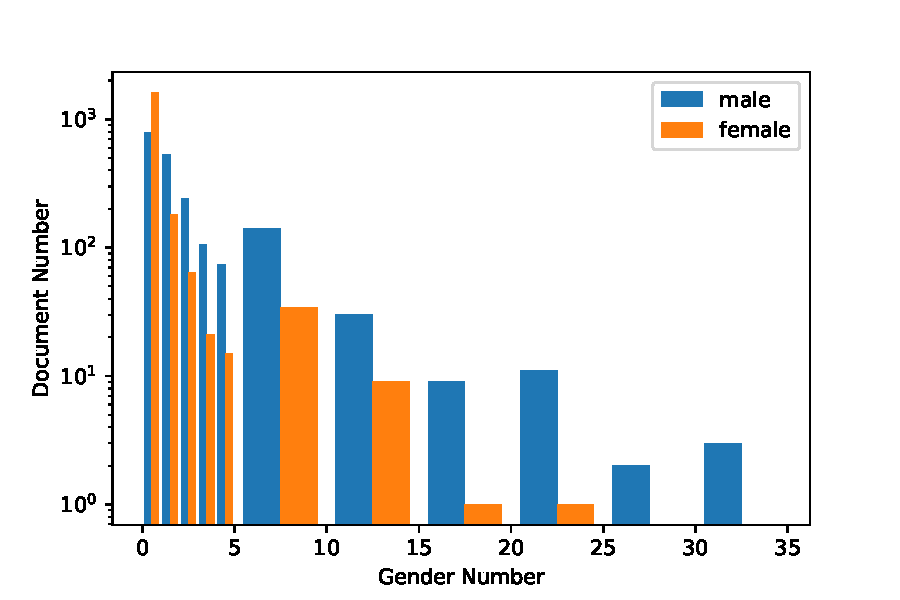
\includegraphics[width=\textwidth]{figures/histogram_cluster_train.pdf}
%         \caption{Histogram of male and female entities in the training set.}
%         \label{fig:his_clu_train}
%     \end{subfigure}~
%     \begin{subfigure}[b]{0.45\textwidth}
%         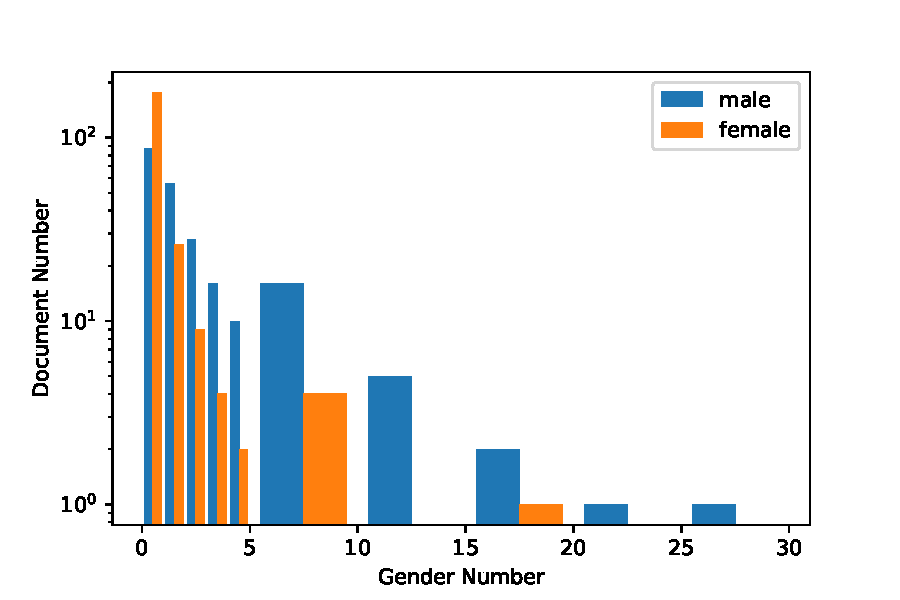
\includegraphics[width=\textwidth]{figures/histogram_cluster_dev.pdf}
%         \caption{Histogram of male and female entities in the development set.}
%         \label{fig:his_clu_dev}
%     \end{subfigure}
%     \caption{Histogram of clusters related to different genders in coreference corpus.
%     % \kw{You want to emphasize the left-most bar represent the number of documents do not have male or female related clusters.}
%     For each document in  training and development dataset, we count how many entities contains male or female pronouns.  The x-axis shows the number of male (blue) and female (orange) entities in each document, y-axis is the number of documents. The left-most bar represents the number of documents  not having any male or female entities. As the results show, there are more documents having no female entities than documents having no male entities. In general, the corpus contains more male entities.}
%     \label{fig:his_cluster}
% \end{figure*}


%  \paragraph{Gender bias associated with job titles.}
%  From the analysis in Table~\ref{tab:words}, we suspect that some job title is associated with male pronoun excursively.
%As the reference to a man or woman also shows stereotype~\cite{BCWS16}, 
%  we analyze how the gender pronouns co-refer with job titles. 
%   To conduct this analysis, 
 
%  We make minor modification on the list to include titles such as ``president''. We report number of times when the job title and the gender pronouns corefer the same entities.
% Results show that there are $776$ male entities are referred by a job title, while only $86$ female entities are referred by a job title in the training corpus.
% This result shows that men are more likely to be referred by their job (e.g., president, leader, CEO).
%  For individual job titles, we observed that there are a few job titles  exclusively refer to male entities.
%  For example, ``leader'' refers to male entities 30 times and is never used to refer female entities.
%  We see the similar trend in the development corpus, where there are $102$ male entitles contains job title mention, and only $14$ female entities are referred by job title.
 
% Given these professional job titles, we will report the ratio of \#(male, job): \#(female, job) in the corpus. Here $\#(a,b)$ stands for how many times $a$ and $b$ co-occurs in the same cluster. 
% The results show that in the training dataset, the gender ratio among all these titles between male and female is $776:86$ which shows whole dataset is extremely biased to male --  with a male ratio about $90\%$.Here the male ratio refers to the ratio of male titles to all the gender titles. For specific job title, the gender ratio also exists. For example, ``leader'', relates to male 30 times in the dataset and 0 times with female while for ``nurse'', the ratio between male and female is 0:2.
%In the development dataset which we will make predictions, we found the dataset is also imbalanced for different genders. In this dataset, we find the gender ratio is $102:14$, around $88\%$ are male. For specific job title, ``lord'' has a ratio 12:0 while the ratio for ``leader'' is 4:0. 

% \paragraph{Different types of genres.}
%We also interested in analyzing if different genres of text have different degree of bias.
%We show the same analysis as above on the seven different types of genre on the OntoNotes 5.0 corpus.
%The results are shown in Table~\ref{tab:subsets}.
%Except for the telephone conversation, all the subsets are biased toward male and the bible is the most biased.
%Without surprise, bible (PT) is the most biased dataset, where most entities are male. 
%News dataset (BN and NW) are also extremely biased toward male, as most political figures are male.
%Besides, some common jobs which occur in most genres  such as ``president '',  ``minister'' and ``teacher'' are all male biased.
%We will show later that the bias in the corpus causes models failing to recognize certain job titles such as prime minister can refer to female entities.\footnote{Several countries, including Norway, Poland, German and the United Kingdom, have female ministers}
%Among all the subsets of data, broadcast news, newswire and pivot text are extremely biased to male, in both dataset having over $90\%$ job titles related to male. Also we notice the job ratio seems more biased than the cluster ratio which may be caused by people  referring to the male by their job titles more often than female. 

% \begin{table*}[thbp]
% \centering
%     \begin{tabular}{l|cc|c c|c|c|c|}
%         \hline
%         \multicolumn{7}{c}{\bf Training Dataset} \\
%         \hline
%          \bf{Genres} 
%          &  \multicolumn{2}{|c|}{\bf{Cluster Ratio}}
%          & \multicolumn{2}{|c|}{\bf{Job Ratio}}
%          & \multicolumn{3}{|c|}{\bf{Common Jobs}} \\ \cline{2-8}
%          & m:f & m\% & m:f & m\% & president & minister & teacher \\
%           \hline
%         Broadcast Conversation (BC)  & 357:87 & 80.4  & 65:14 & 82.3 & 29:1 & 2:0 &  0:2\\
%          \hline
%         Broadcast News (BN) & 613:114 & 84.3 & 175:15 & 92.1 & 63:1 &  18:0 & 0:1 \\
%         \hline
%         Magazine (MZ) & 353:149 & 70.3 & 37:14 & 72.5 &  7:2 &  0:1 & 1:1  \\
%         \hline
%         Newswire (NW) & 703:103 & 87.2 & 141:15  & 90.4 & 22:0 & 4:1  &  0:0 \\
%         \hline
%         Telephone Conversation (TC)  & 140:156 & 47.3 & 8:10 & 44.4 & 1:0 & 0:0 & 0:1 \\
%         \hline
%         Weblogs and Newsgroup (WB) & 306:66 & 82.2& 61:4 & 93.8 & 5:0 & 5:0 & 1:0  \\
%         \hline
%         Pivot Text [PT] (New Testament) & 921:112 & 89.2 & 289:14 & 95.4 & 0:0 & 0:0 & 31:0 \\
%         \hline
%         Total Dataset & 3393:787 & 81.2& 776:86 & 90.0 & 127:4 & 29:2 & 33:5 \\
%         \hline
%          \multicolumn{7}{c}{\bf Development Dataset} \\
%         \hline
%          \bf{Genres} 
%          &  \multicolumn{2}{|c|}{\bf{Cluster Ratio}}
%          & \multicolumn{2}{|c|}{\bf{Job Ratio}}
%          & \multicolumn{3}{|c|}{\bf{Common Jobs}} \\ \cline{2-8}
%          & m:f & m \% & m:f & m\% & president & minister & teacher \\
%           \hline
%         Broadcast Conversation (BC)  &  68:28 & 70.8 &17:7 & 70.8 & 0:0 & 0:0 & 0:0 \\
%          \hline
%         Broadcast News (BN) & 87: 15 &85.3 & 17:0  &100  &9:0  & 0:0 &  0:0 \\
%         \hline
%         Magazine (MZ) & 43:6 & 87.8 & 4:0 & 100 & 4:0 & 0:0  & 0:0  \\
%         \hline
%         Newswire (NW) & 109:16 & 87.2 & 33:1 & 97.1 & 7:1  &  1:0 &   0:0 \\
%         \hline
%         Telephone Conversation (TC)  &16:26 & 38.1 & 0:3 & 0 &0:0 & 0:0 & 0:0  \\
%         \hline
%         Weblogs and Newsgroup (WB) &  40:12 & 76.9 & 6:3  & 66.7 & 0:0 & 0:0 & 0:1  \\
%         \hline
%         Pivot Text [PT] (New Testament) & 78:8 & 90.7 & 25:0 & 100& 0:0 & 0:0 & 6:0 \\
%         \hline
%         Total Dataset & 441:111 & 79.9 & 102:14 & 87.9 & 20:0 & 1:0 & 6:1 \\
%         \hline
%     \end{tabular}
%     \caption{Gender bias in different genres. Here $m:f$ refers to the total numbers of male and female entities on the dataset. See text for the detailed definition. $m\%$ stands for the male ratio among all the gender related items (i.e., $m/(m+f)$).  }
%     \label{tab:subsets}
% \end{table*}
% \begin{table*}[thbp]
% \centering
%     \begin{tabular}{|l|cc|c c|cc|}
%         \hline
%         \multicolumn{7}{c}{\bf Training Dataset} \\
%         \hline
%          \bf{Genres} 
%          &  \multicolumn{2}{c|}{\bf{Cluster Ratio}}
%          & \multicolumn{2}{c|}{\bf{Job Ratio}}
%          & \multicolumn{2}{c|}{\bf{Common Jobs}} \\ \cline{2-7}
%          & m:f & m\% & m:f & m\% & m:f & m\%  \\
%           \hline
%         Broadcast Conversation (BC)  & 357:87 & 80.4  & 65:14 & 82.3 & 31:3 & 91.2\\
%          \hline
%         Broadcast News (BN) & 613:114 & 84.3 & 175:15 & 92.1 &81:2 & 97.6\\
%         \hline
%         Magazine (MZ) & 353:149 & 70.3 & 37:14 & 72.5  & 8:4 & 66.7\\
%         \hline
%         Newswire (NW) & 703:103 & 87.2 & 141:15  & 90.4 & 26:1 & 96.3 \\
%         \hline
%         Telephone Conversation (TC)  & 140:156 & 47.3 & 8:10 & 44.4 & 1:1 & 50\\
%         \hline
%         Weblogs and Newsgroup (WB) & 306:66 & 82.2& 61:4 & 93.8 & 11:0 & 100 \\
%         \hline
%         Pivot Text [PT] (New Testament) & 921:112 & 89.2 & 289:14 & 95.4 & 31:0 & 100 \\
%         \hline
%         Total Dataset & 3393:787 & 81.2& 776:86 & 90.0 & 193:11 & 94.6 \\
%         \hline

%     \end{tabular}
%     \caption{Gender bias in different genres. Here $m:f$ refers to the total numbers of male and female entities on the dataset. See text for the detailed definition. $m\%$ stands for the male ratio among all the gender related items (i.e., $m/(m+f)$). The ``common jobs'' here refer to the three jobs appearing in most genres.}
%     \label{tab:subsets}
% \end{table*}

% \subsection{Coreference Resolution Systems are Biased}
% \paragraph{Coreference Resolution Systems are Biased}
% % From the above analysis we can see that both the training and the  development datasets are biased toward male. 
% From the above analysis we can see that the corpus is biased toward male, when training a model on such corpus, the model inherits the bias and makes systematic mistakes.
% For example, ``the president'' refers to male entities 127 times while only refers to female entities 4 times. Therefore, the model learns that ``the president'' is associated with male pronouns and fail to recognize female presidents. As a result, the model makes a biased prediction as shown in the example in Fig.~\ref{fig:president}. 
%If we build decision system based on the model or even just using the datasets, there will be potentials that we make mistake about the underneath truth.
%As  the example in Fig.~\ref{fig:president}, if the coreference resolution systems are gender fair, they should have the ability to refer ``her'' to the ``president'' which is not the case.
% To show coreference systems making gender-biased decisions, we conduct the following procedure. 
% % We first evaluate the model on the original development dataset.  
% We  generate a gender-reversed development corpus by exchanging male and female pronouns. If the model is gender neural, the performance of the system should not be affected much by the changes of gender pronouns. Therefore, by comparing the performances on the original and on the gender-reversed corpora, we can estimate how the model is sensitive to the gender of entities.

%then adopt the model on  the gender-reversed development dataset we build and compare the performance with the previous results. This new  dataset will have different gender information comparing to the original one. If the performance drops, it means the system takes ``he'' and ``she'' very differently, indicating the gender bias. 

% \textbf{ Building the gender-reversed datasets.}
%The gender-reversed dataset  reduces the gender information in the original datasets. Based on these datasets we can testify the original model's ability to tell the difference between man and woman. What we do is that 
% We first collect a list of word pairs represent male and female, such as  
%  ``woman''-``man'', ``she''-``he'', and ``her''-``his''.\footnote{We use the list generated from word embeddings by \cite{BCWS16}. The list can be download at \url{https://github.com/tolga-b/debiaswe/blob/master/data/definitional\_pairs.json}}. We then exchange the female word and male word in the corpus based on the list. In this way, we generate a gender-reversed corpus. 

% To build the gender-reversed datasets, we asked Amazon Mechanical Turk to identify if a span in the coreference chain is related to male or female. If it is , we then ask them to exchange it to the corresponding span with the other gender. For example, ``a waiter'' in the original corpus will be changed to ``a waitress'' in the new dataset. To get rid of the influence of names, we first anonymize the whole dataset.



 %We then replace all the female-related words to the corresponding male-related words and vice versa. By now we generate the gender-reversed dataset. 
% The gender-reversed corpus can be used as a proxy to understand how the model is sensitive to the gender of entities. However, this approach has some deficit. If an entity is originally referred by a female name and a female pronoun, after  we exchange the female pronoun to a male pronoun, the male pronoun has to refer to the female name. However, we find this situation is not frequent. The most frequent male name  ``Paul'' in the training corpus only appears in 47 clusters while ``Mary'' appears in only 15 clusters. As there are more than 35,000 entities in the training corpus, this effect can be neglected. 
%Comparing to more than 35,000 clusters in the training dataset we think the name situation does not happen very frequently.~\footnote{``Clinton'' relates to both male and female, but here we only talk about the exclusively male and female name.} In fact in the word list from paper~\cite{BCWS16}, they also have a pair of male and female name like ``Mary '' and ``John''.
%We can see in the following that the performance on the reversed development dataset is much worse than on the original development dataset. 
% \textbf{Performance Evaluation.} 
% \kw{You can remove the following paragraph. All the model should use the same evaluation method, and you should mention it in Sec 2}
% We show the performance for various coreference resolution systems on the original and the gender-reversed datasets in Table~\ref{tab:bias}.

%decrease in performance means when we reverse the gender pronoun in the dataset, the model no longer makes good predictions as shown in Fig.~\ref{fig:president}.  This is caused by the model taking male and female differently. Previous related entities no longer predicted in the same cluster indicates the gender bias.
% We also conduct the experiments on the unseen test corpus and observe the same trend. Despite Stanford, Berkeley, and UW coreference systems are different in nature, they all potentially make gender-biased decisions.
% \kw{The readers will not get the meaning of performance drops in gender-reversed data. So you have to give some explanation why performance drops in the gender-reversed data means there is gender bias.}
%The results  show the same falling trend, which means the rule-based, feature-based and even state-of-the-art neural network system all potentially have the gender bias issue.

% \begin{table}[t]
% \centering
%     \begin{tabular}{|l|c|c|}
 
%         \hline
%          \bf System & \bf  Original Perf.& \bf Gender-reversed  Perf.\\
%           \hline
%           \multicolumn{3}{|c|}{Development Set} \\
%           \hline
%         CoreNLP  &   56.98   &  54.40 \\
%          \hline
%         Berkeley &  61.71  &  60.13 \\
%         \hline
%         UW e2e  &   67.70  & 66.44   \\
%         \hline
%         \multicolumn{3}{|c|}{Test Set} \\
%           \hline
%         CoreNLP  &  55.6   &  53.39 \\
%          \hline
%         Berkeley &  61.2  &  60.58 \\
%         \hline
%         UW e2e  &   67.22  &  65.64   \\
%         \hline  
%     \end{tabular}
%     \caption{ Performance of various systems on the original and the gender-reversed corpus. ``Original Perf.'' stands for the model's performance on the original dataset. ``Gender-reversed Perf.'' refers to the model's performance on the dataset where male and female mentions are exchanged.
%     }
%     \label{tab:bias}
% \end{table}



% \textbf{Gender Imbalanced in the Predictions.}
% % \kw{Need to give some motivations. Why we want to analyze job title?}
% We are interested in analyzing if the coreference predictions are gender imbalanced. We conduct a similar analysis as in Section \ref{sub:ccb}. 
% We shows the number of male and female entities and how the job titles associated with the male and female entities on the predicted coreference clustering.

% We first consider the system predicted coreference clustering on the original corpus. In the coreference clustering generated by Berkeley system, there are 71 male entities referred by a job title, while only 8 female entities referred by a job. Comparing to the ground true, where the ratio is $102:14$, the ratio of male referred by job title increases. In fact, except ``cook'' and ``mother'', all the other $26$ job titles are related to male entities. The UW system demonstrates the same trend, where there are 48 and 9 male and female entities referred by a job title, respectively. The prediction is less biased and system performance is better. 


% Taking Berkeley system as an example,
%when predicting on the original development dataset, the result is imbalanced: the predicted ratio for these job titles is $71:8$ which shows $2\%$ more male bias, comparing to the ground truth ratio $102:14$. There are in total $28$ different job titles in the prediction, but only ``cook'' and ``mother'' are related to female, which also implies the gender bias. 

% \kw{need to explain what is the prediction ratio means. Both the mathmatical definition and the underlying meaning.}

% Also the prediction seems to have little relation with female. While we acknowledged that the dataset is not that large, but among the whole predictions from Berkeley system, even though there are totally 28 job titles, only 2 out of them are related to female, which are ``cook'' and ``mother'', which also implies the gender bias.



%And for UW e2e system, the predicted gender ratio is $48:9$ showing less bias than Berkeley system but also fewer predicted job titles. There are in total 25 job titles in prediction, and 4 of them are related to female. 

% \paragraph{Predictions on the gender-reversed development dataset.}
% If the coreference resolution systems are gender neutral, when making a prediction on the gender reversed dataset, they should get the exactly reversed gender ratio. However, the analysis shows a great gap between the predictions from the gender reversed and the original datasets.
% For specific job title, such as ``president'', the ground truth ratio is $20:0$.  The predicted ratio by Berkeley system in original development dataset is $18:0$ which is close to the ground truth. But when predicting on the reversed dataset, it becomes $0:7$, which means the model cannot capture the coreference between ``president'' and female. 
% In UW e2e system, the gender ratio for ``president '' in the original dataset is $10:0$ and $1:8$ in the gender-reversed dataset. The UW system seems to have less bias than Berkeley system but it also predicts fewer titles.

% The gap between the predicted ratio in the original  and the gender reversed dataset also explains the  performance decrease in the above section.



% \jy{
% We test the UW model on the swapped subset. Basically we collect the sentences with some gender swapped by the Turk. 

% \begin{table*}[t]
% \centering
%     \begin{tabular}{|l|c|c|}
 
%         \hline
%          \bf Retrained Model & \bf  Performance on the swapped sub-dataset& \bf Performance on the unswapped sub-dataset \\
%           \hline
         
%         Only\_on\_anonymized dataset  &  63.51   &  65.67 \\
%          \hline
%         Anonymized+swapped(using list from Mark's swapping) &  64.69  &  64.88 \\
%         \hline
%     \end{tabular}
%     \caption{ Performance for different model on the swapped subset.
%     }
%     \label{tab:bias}
% \end{table*}

% }

